
%%%%%%%%%%%%%%%%%%%%%%%%%%%%% Define Article %%%%%%%%%%%%%%%%%%%%%%%%%%%%%%%%%%
\documentclass[conference]{IEEEtran}
%%%%%%%%%%%%%%%%%%%%%%%%%%%%%%%%%%%%%%%%%%%%%%%%%%%%%%%%%%%%%%%%%%%%%%%%%%%%%%%

%%%%%%%%%%%%%%%%%%%%%%%%%%%%% Using Packages %%%%%%%%%%%%%%%%%%%%%%%%%%%%%%%%%%
\usepackage{geometry}
\usepackage{graphicx}
\usepackage{amssymb}
\usepackage{amsmath}
\usepackage{amsthm}
\usepackage{empheq}
\usepackage{mdframed}
\usepackage{booktabs}
\usepackage{lipsum}
\usepackage{graphicx}
\usepackage{color}
\usepackage{psfrag}
\usepackage{pgfplots}
\usepackage{bm}
\usepackage[spanish]{babel}
\usepackage[utf8]{inputenc} % Codificación UTF,8
\usepackage{amsmath}        % Soporte para ecuaciones matemáticas
\usepackage{graphicx}       % Manejo de imágenes
\usepackage{hyperref}       % Hipervínculos
\usepackage{caption}        % Formato para figuras
\usepackage{multirow}
\usepackage{subcaption}
\usepackage{biblatex}
\addbibresource{ref/cable.bib} % Add the bibliography file in the preamble (correct usage)
\usepackage{csquotes}
\usepackage{bookmark}
%%%%%%%%%%%%%%%%%%%%%%%%%%%%%%%%%%%%%%%%%%%%%%%%%%%%%%%%%%%%%%%%%%%%%%%%%%%%%%%

% Other Settings

%%%%%%%%%%%%%%%%%%%%%%%%%% Page Setting %%%%%%%%%%%%%%%%%%%%%%%%%%%%%%%%%%%%%%%
\geometry{a4paper, margin=1in}

%%%%%%%%%%%%%%%%%%%%%%%%%% Define some useful colors %%%%%%%%%%%%%%%%%%%%%%%%%%
\definecolor{ocre}{RGB}{243,102,25}
\definecolor{mygray}{RGB}{243,243,244}
\definecolor{deepGreen}{RGB}{26,111,0}
\definecolor{shallowGreen}{RGB}{235,255,255}
\definecolor{deepBlue}{RGB}{61,124,222}
\definecolor{shallowBlue}{RGB}{235,249,255}
%%%%%%%%%%%%%%%%%%%%%%%%%%%%%%%%%%%%%%%%%%%%%%%%%%%%%%%%%%%%%%%%%%%%%%%%%%%%%%%

%%%%%%%%%%%%%%%%%%%%%%%%%% Define an orangebox command %%%%%%%%%%%%%%%%%%%%%%%%
\newcommand\orangebox[1]{\fcolorbox{ocre}{mygray}{\hspace{1em}#1\hspace{1em}}}
%%%%%%%%%%%%%%%%%%%%%%%%%%%%%%%%%%%%%%%%%%%%%%%%%%%%%%%%%%%%%%%%%%%%%%%%%%%%%%%

%%%%%%%%%%%%%%%%%%%%%%%%%%%% English Environments %%%%%%%%%%%%%%%%%%%%%%%%%%%%%
\newtheoremstyle{mytheoremstyle}{3pt}{3pt}{\normalfont}{0cm}{\rmfamily\bfseries}{}{1em}{{\color{black}\thmname{#1}~\thmnumber{#2}}\thmnote{\,,,\,#3}}
\newtheoremstyle{myproblemstyle}{3pt}{3pt}{\normalfont}{0cm}{\rmfamily\bfseries}{}{1em}{{\color{black}\thmname{#1}~\thmnumber{#2}}\thmnote{\,,,\,#3}}
\theoremstyle{mytheoremstyle}
\newmdtheoremenv[linewidth=1pt,backgroundcolor=shallowGreen,linecolor=deepGreen,leftmargin=0pt,innerleftmargin=20pt,innerrightmargin=20pt,]{theorem}{Theorem}[section]
\theoremstyle{mytheoremstyle}
\newmdtheoremenv[linewidth=1pt,backgroundcolor=shallowBlue,linecolor=deepBlue,leftmargin=0pt,innerleftmargin=20pt,innerrightmargin=20pt,]{definition}{Definition}[section]
\theoremstyle{myproblemstyle}
\newmdtheoremenv[linecolor=black,leftmargin=0pt,innerleftmargin=10pt,innerrightmargin=10pt,]{problem}{Problem}[section]
%%%%%%%%%%%%%%%%%%%%%%%%%%%%%%%%%%%%%%%%%%%%%%%%%%%%%%%%%%%%%%%%%%%%%%%%%%%%%%%

%%%%%%%%%%%%%%%%%%%%%%%%%%%%%%% Plotting Settings %%%%%%%%%%%%%%%%%%%%%%%%%%%%%
\usepgfplotslibrary{colorbrewer}
\pgfplotsset{width=8cm,compat=1.9}
%%%%%%%%%%%%%%%%%%%%%%%%%%%%%%%%%%%%%%%%%%%%%%%%%%%%%%%%%%%%%%%%%%%%%%%%%%%%%%%

%%%%%%%%%%%%%%%%%%%%%%%%%%%%%%% Title & Author %%%%%%%%%%%%%%%%%%%%%%%%%%%%%%%%
\author{\IEEEauthorblockN{Daniel Fernando Aranda Contreras, Diana Fernanda Abril Roa, Nicolás Hernández Buitrago,\\ Rafael Miguel Segura Garzon}
\IEEEauthorblockA{Escuela E3T, Universidad Industrial de Santander\\
Correo electrónico: \{daniel2221648, diana2212074, nicolás2204593, rafael2202194 \}@correo.uis.edu.co}}

%%%%%%%%%%%%%%%%%%%%%%%%%%%%%%%%%%%%%%%%%%%%%%%%%%%%%%%%%%%%%%%%%%%%%%%%%%%%%%%
    \begin{document}
        % Título
        \title{\uppercase{Diseño y construcción de un transformador eléctrico}}
        \maketitle
        % Resumen
        % Palabras clave        
        \begin{IEEEkeywords}
            Transformador
            Tensión,
            Bobinado,
            Relación de transformación,
            Aislante,
            Fusibles,
            Corriente,
            Potencia,
            Diseño,
            Construcción.
        \end{IEEEkeywords}


        %\section{Objetivos} 
\begin{itemize}
    \item Realizar las pruebas de vacío y de cortocircuito en un transformador monofásico configurado como autotransformador para analizar su comportamiento eléctrico.
    \item Determinar experimentalmente el rendimiento y la regulación del autotransformador bajo diferentes tipos de carga: resistiva, inductiva y capacitiva.
\end{itemize}

\section{Equiops y materiales}
\begin{itemize}
    \item Transformador monofásico.
    \item Voltímetro CA.
    \item Amperímetro CA.
    \item Vatímetro monofásico CA.
    \item Transformador de corriente (CT).
    \item Cargas: resistivas (R), inductivas (L) y capacitivas (C).
\end{itemize}

\section{Introducción}
\text{Los autotransformadores son dispositivos eléctricos que facilitan la modificación de los niveles de tensión dentro de un rango específico de manera eficiente. A diferencia de los transformadores tradicionales, en los autotransformadores los devanados primario y secundario no están completamente aislados, ya que comparten una parte del mismo arrollamiento. Esto resulta en una reducción del material conductor utilizado y en una mejora de la eficiencia del sistema. En este laboratorio, se realizará un estudio de un transformador monofásico funcionando como autotransformador, a través de pruebas experimentales que permitirán evaluar su rendimiento y regulación en diversas condiciones de carga.}

\section{Conclusión}
\text{A lo largo del laboratorio, se estudió el comportamiento de un transformador monofásico operando como autotransformador, evaluando su rendimiento y regulación bajo diferentes condiciones de carga, las cuales tienen una gran influencia en su rendimiento depediendo el tipo de carga, si es una carga RC conectada en paralelo tiende a aunmentar su tension de salida en comparacion con una carga netamente resistiva, mientras que con una carga inductiva conectada en serie su nivel de tension de salida disminuye, pero si conectamos una carga RLC está tiene un comportamiento de compensacion, si las cargas inductivas (L) y capacitivas (C) tienen valores similares.}
        \section{Objetivos}

\begin{itemize}
    \item Identificar correctamente los bornes de conexión y los devanados internos (de campo y de armadura) de una máquina de corriente continua, con base en su configuración eléctrica y esquema de conexión.
    \item Medir la resistencia de aislamiento de los devanados de la máquina de C.C. utilizando un megóhmetro, verificando su estado eléctrico conforme a los estándares de seguridad eléctrica.
    \item Determinar la caída de tensión en las escobillas durante el funcionamiento de la máquina, evaluando su condición operativa y su influencia en el rendimiento del equipo.
    \item Desarrollar habilidades prácticas en el uso de instrumentos de medición eléctrica aplicados al diagnóstico y análisis de máquinas de corriente continua.
\end{itemize}

\section{Equipos y Materiales}

\begin{itemize}
    \item Máquinas de corriente continua.
    \item Megóhmetro (Megger).
    \item Ohmímetro.
    \item Voltímetro.
    \item Amperímetro.
\end{itemize}

\section{Introducción}

Las máquinas de corriente continua (C.C.) son equipos electromecánicos ampliamente utilizados en aplicaciones donde se requiere un control preciso de la velocidad y el par. Estas máquinas pueden clasificarse, según su tipo de excitación, en tres categorías principales: máquinas en derivación (shunt), en serie y compuestas (compound). Cada una presenta características de operación particulares que las hacen adecuadas para distintas condiciones de carga y aplicaciones industriales.

 Antes de poner en funcionamiento una máquina eléctrica nueva, reparada o que haya estado inactiva, es fundamental realizar una serie de pruebas preliminares que garanticen su correcto funcionamiento y la seguridad durante la operación. Estas pruebas incluyen la identificación y verificación de los bornes de conexión, la medición de la resistencia eléctrica de los devanados, la evaluación de la resistencia de aislamiento, la determinación de la caída de tensión en las escobillas y, en ciertos casos, la comprobación de la zona neutra geométrica. Estas verificaciones permiten prevenir fallos eléctricos, evitar daños en los componentes y asegurar que la máquina cumpla con los estándares técnicos y normativos vigentes.
 Esta práctica de laboratorio tiene como finalidad aplicar estos procedimientos de diagnóstico en una máquina de corriente continua, desarrollando habilidades en el manejo de instrumentos de medición y fortaleciendo la comprensión del comportamiento eléctrico y mecánico de este tipo de máquinas. 
        \section{MARCO TEÓRICO}
Las máquinas de corriente continua (CC) son dispositivos electromecánicos que convierten energía eléctrica en energía mecánica (motores) o viceversa (generadores). Aunque en la actualidad han sido en gran parte reemplazadas por máquinas de corriente alterna en muchas aplicaciones, las máquinas de CC siguen siendo fundamentales en entornos industriales, sistemas de control, vehículos eléctricos y laboratorios educativos, debido a su capacidad de control preciso de velocidad y torque.\newline

Una máquina de corriente continua está compuesta principalmente por un \textbf{estator}, que proporciona el campo magnético, y un \textbf{rotor} o \textbf{armadura}, que gira dentro de ese campo. El intercambio de corriente entre la armadura giratoria y el circuito externo se logra mediante el \textbf{conmutador} y las \textbf{escobillas}, lo que permite mantener una dirección unidireccional de la corriente en el circuito externo, incluso cuando la máquina está en movimiento.\newline

Las \textbf{medidas preliminares} en el estudio de una máquina de CC son esenciales para garantizar un funcionamiento seguro y eficaz antes de realizar ensayos más exigentes. Estas medidas incluyen la \textbf{resistencia de los devanados del inducido y del campo}, la \textbf{verificación de la polaridad}, la \textbf{identificación de terminales}, la \textbf{comprobación de la continuidad}, y la \textbf{inspección visual de conexiones y escobillas}. Estas pruebas permiten detectar fallas como cortocircuitos, circuitos abiertos o conexiones incorrectas, que podrían afectar el rendimiento de la máquina o provocar daños durante su operación.\newline

Comprender el comportamiento eléctrico básico de la máquina en estado de reposo (sin carga) permite también establecer una línea base para futuros análisis de desempeño, eficiencia y respuesta dinámica. Además, estas mediciones son cruciales para el desarrollo de modelos matemáticos que representen la máquina en simulaciones o aplicaciones de control.\newline




        \section{Actividad}

\subsection*{Identificación de devanados:}

Es necesario realizar algunas medidas preliminares. Estas comprenden la identificación de los bornes y verificación de su marcación. En este laboratorio se tomarán estas respectivas medidas de las máquinas de corriente continua que se encuentran en el laboratorio de Máquinas 1: Shunt y Compound.
\begin{figure}[ht!]
    \centering
    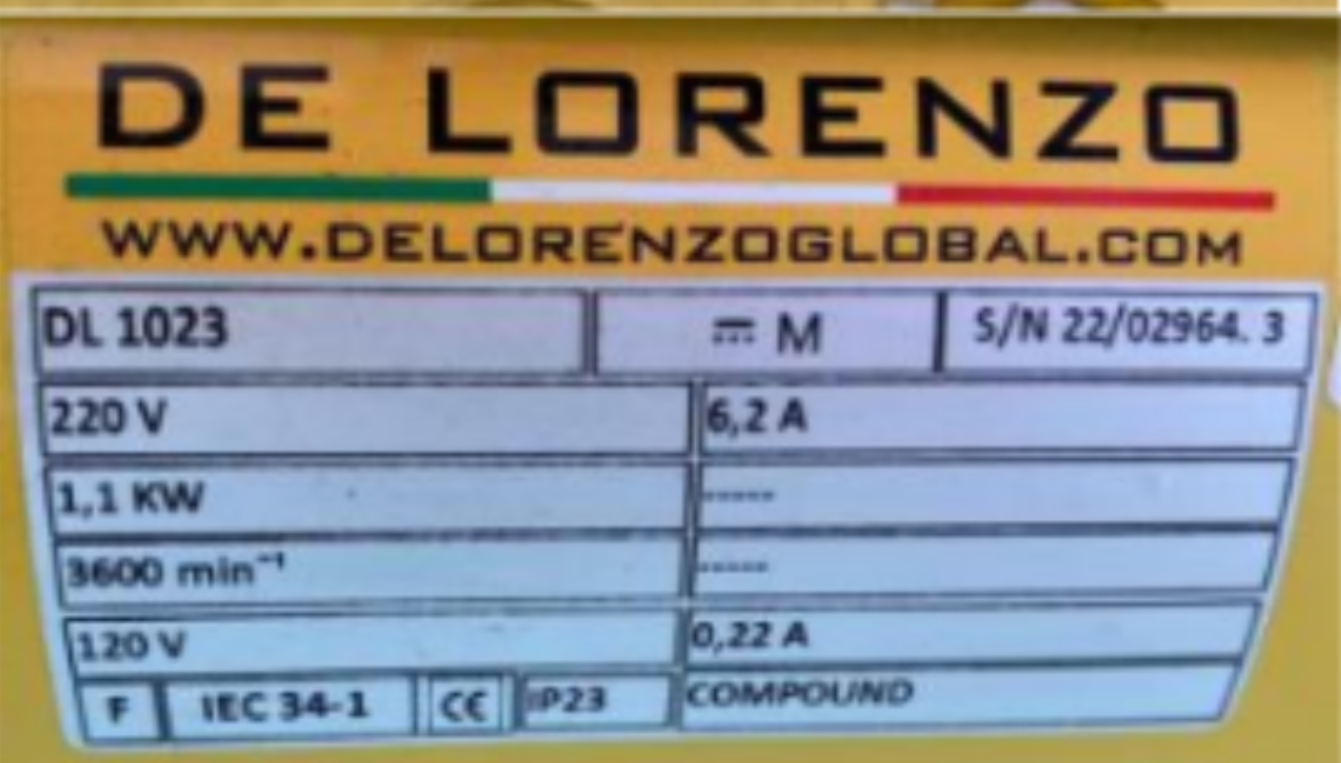
\includegraphics[width=0.48\textwidth]{fot/Prac_6_compound.png}
    \caption{Motor compound del laboratorio.}
    \label{fig:compound}
\end{figure}
\begin{figure}[ht!]
    \centering
    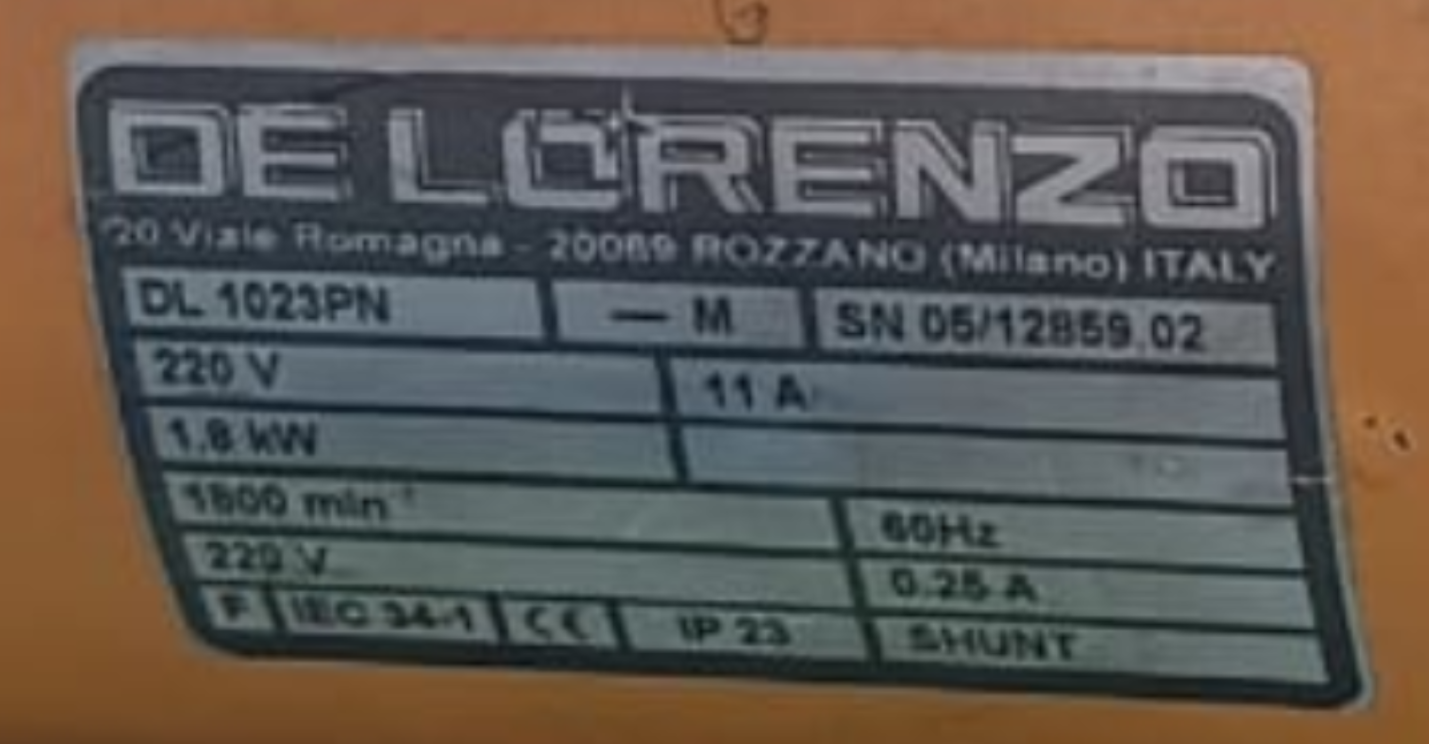
\includegraphics[width=0.48\textwidth]{fot/Prac_6_shunt.png}
    \caption{Motor shunt del laboratorio.}
    \label{fig:shunt}
\end{figure}
Para la identificación de los bornes usaremos un multímetro con el que podremos verificar la continuidad de cada uno de los bornes, con eso sabremos cuáles son los bornes a los que tendremos que medirles su valor resistivo. Para identificarlos, tendremos que tener los siguientes puntos en cuenta:

\begin{itemize}
    \item El devanado de campo shunt tiene el mayor valor resistivo de todos los devanados.
    
    \item El devanado de armadura se hace girar el eje, porque si en los bornes medidos se induce tensión, así sea un poco, ese sería el devanado de armadura.
    
    \item Para este devanado teníamos también acceso a las escobillas, con este también se podría identificar directamente.
    
    \item Para identificar el devanado de campo serie se tiene que aplicar unos pulsos en el devanado shunt y donde se encuentre la mayor tensión en los devanados no identificados, ese sería el devanado de campo serie.
\end{itemize}

Este procedimiento se realizará para cada una de las máquinas que tenemos en el laboratorio: Shunt, Compuesta. Como la identificación de los bornes no requiere de procedimientos complejos, los instrumentos y equipos que usaremos en el laboratorio serán un multímetro.

\subsection*{Resistencia en los devanados (shunt)}

\begin{tabular}{|c|c|c|}
\hline
DEVANADO & VALOR ($\Omega$) & BORNES \\
\hline
ARMADURA & 3.5 & A1-B2 \\
SHUNT & 8.77 & E1-E2 \\
\hline
\end{tabular}

\subsection*{Resistencia de aislamiento (shunt)}

\begin{tabular}{|c|c|c|}
\hline
VALOR (G$\Omega$) & BORNES \\
\hline
7.45 & A1 - TIERRA \\
926 & E2 - TIERRA \\
5.49 & B2 – E2 \\
\hline
\end{tabular}

\subsection*{Resistencia en los devanados (Compound)}

\begin{tabular}{|c|c|c|}
\hline
DEVANADO & VALOR ($\Omega$) & BORNES \\
\hline
ARMADURA & 2.7 & A1 – B2 \\
SERIE & 0.5 & D1 – D2 \\
SHUNT & 0.570 (k) & E1 – E2 \\
\hline
\end{tabular}

\subsection*{Resistencia de aislamiento (Compound)}

\begin{tabular}{|c|c|c|}
\hline
VALOR (G$\Omega$) & BORNES \\
\hline
18.8 & A1 - TIERRA \\
20.9 & D1 - TIERRA \\
4.75 & E1 – TIERRA \\
4.93 & A1 – D1 \\
1.94 & A1 – E1 \\
4.47 & D1 – E1 \\
\hline
\end{tabular}

Para la siguiente parte del laboratorio usaremos el esquema que se nos indicó en la guía de la práctica, el cual es tomar el voltaje y corriente del devanado de armadura (Ra, Va, Ia) con eso generar una tabla y esa misma tabla se extrapolará para poder encontrar el valor aproximado de la caída de tensión en las escobillas.

El esquema que se piensa usar es el siguiente (figura \ref{fig:modelol}).
\begin{figure}[ht!]
    \centering
    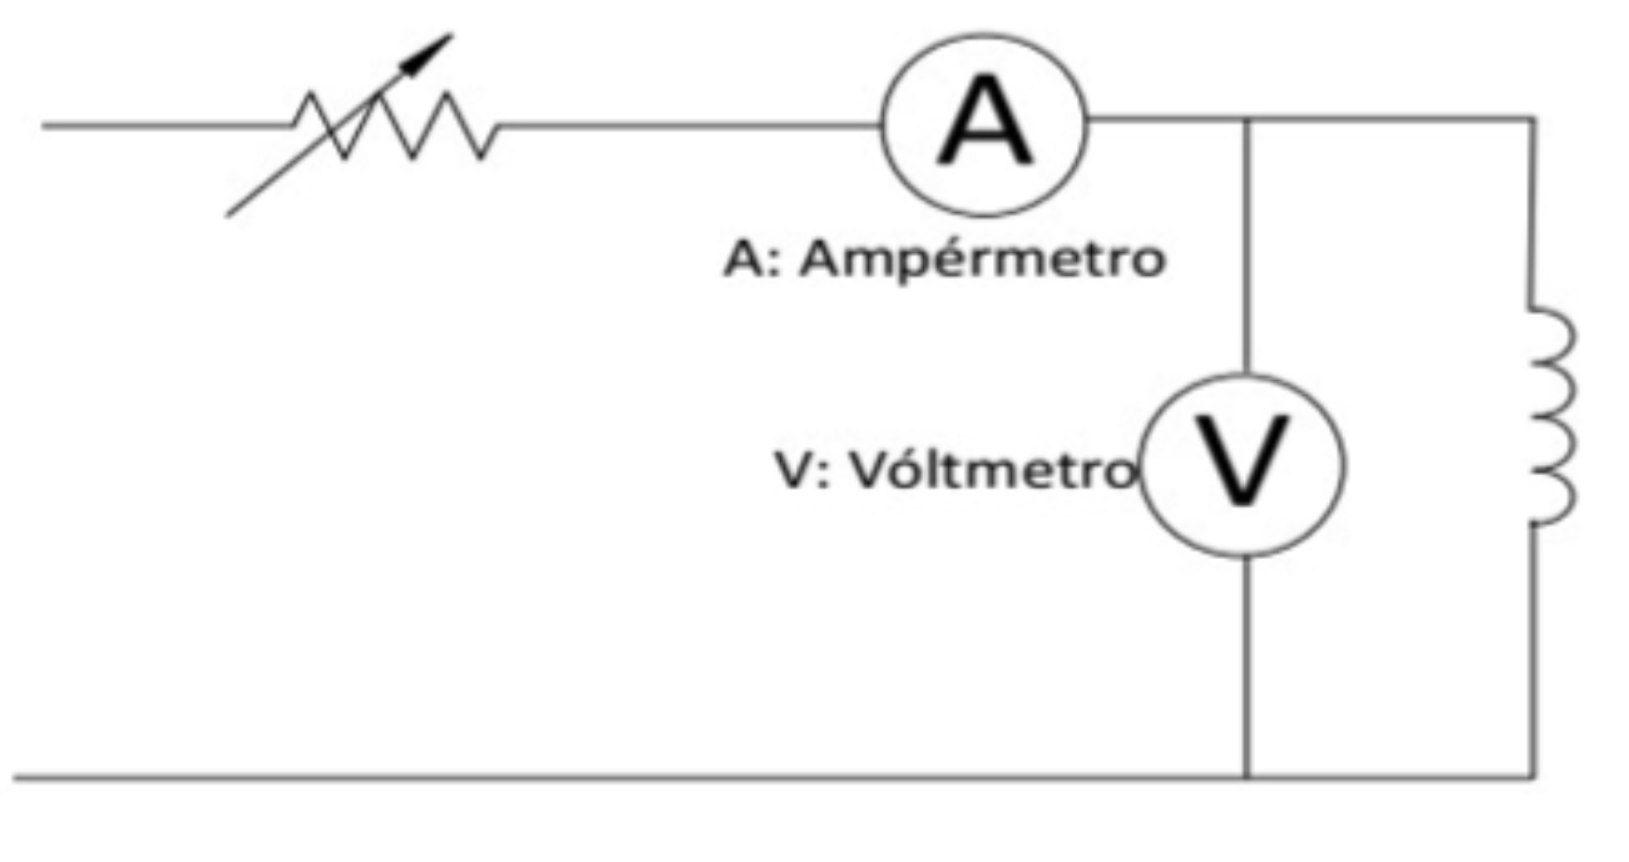
\includegraphics[width=0.48\textwidth]{fot/Prac_6_modelo.png}
    \caption{Topologia de circuito usada para el equivalente.}
    \label{fig:modelol}
\end{figure}


\begin{tabular}{|c|c|c|}
\hline
RESISTENCIA ($\Omega$) & VOLTAJE (V) & CORRIENTE (A) \\
\hline
Máxima & 1.36 & 0.8 \\
2 & 2.020 & 1 \\
3 & 3.560 & 1.49 \\
4 & 5.770 & 2.07 \\
5 (mínima) & 10.93 & 3.60 \\
\hline
\end{tabular}

Con los datos obtenidos anteriormente en la tabla 1, podremos construir la figura \ref{fig:grafica}.
\begin{figure}[ht!]
    \centering
    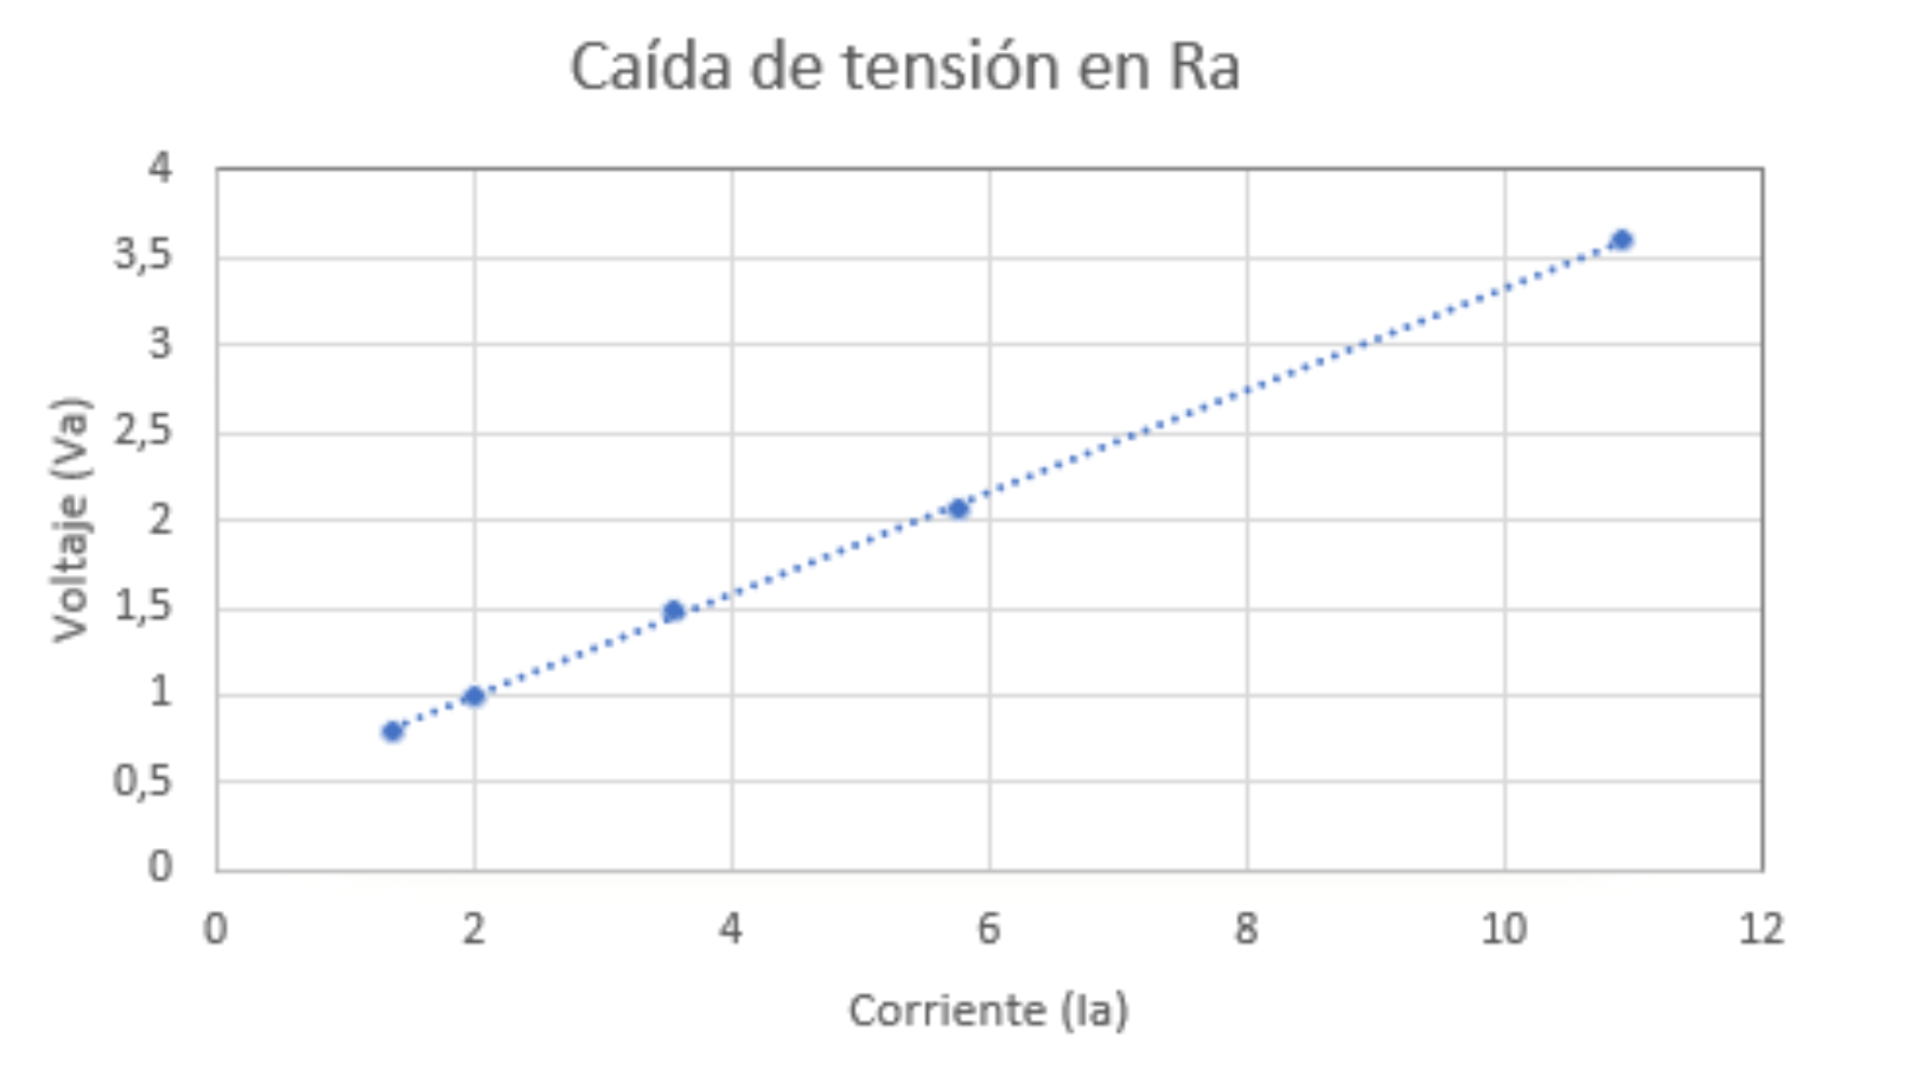
\includegraphics[width=0.48\textwidth]{fot/Prac_6_graf.png}
    \caption{extrapolación de los datos y así obtener la caída de tensión en las escobillas.}
    \label{fig:grafica}
\end{figure}

\textit{Imagen. Gráfica caída de tensión en Ra}

Haciendo la extrapolación con los datos obtenidos y analizándolos de forma lineal, podremos conseguir la caída de tensión en escobillas.

Caída de tensión en escobillas: 0.415518 V

\subsection*{¿Qué es la zona neutra geométrica?}
La zona neutra geométrica en una máquina eléctrica, como un generador o motor de corriente continua (DC), se refiere al área específica del conmutador donde la corriente inducida en los conductores del rotor (inducido) cambia de dirección. Es un concepto crucial para la correcta conmutación y operación de la máquina.
\subsubsection*{Características de la Zona Neutra Geométrica:}
\begin{itemize}
    \item \textbf{Ubicación:} La zona neutra geométrica se encuentra en el plano perpendicular al eje del flujo magnético principal generado por el campo de la máquina. Es decir, está en el lugar donde el flujo magnético es teóricamente cero.
    
    \item \textbf{Función:} En esta zona, las escobillas del motor o generador deben estar posicionadas para que no haya una fuerza electromotriz (fem) inducida en los conductores del inducido cuando están en contacto con las escobillas. Esto reduce las chispas y el desgaste en el conmutador y las escobillas.
    
    \item \textbf{Cambio de dirección de corriente:} A medida que el rotor gira, los conductores pasan por la zona neutra geométrica, cambiando la dirección de la corriente. Este cambio debe ser suave para evitar arcos eléctricos y desgaste prematuro.
\end{itemize}

        \section{Conclusiones}
\label{sec:conclusiones}

\begin{itemize}
    \item La identificación correcta de los bornes en máquinas tipo Shunt y Compound permitió una conexión segura y adecuada para las pruebas posteriores, evitando errores comunes que podrían provocar fallas o daños en el equipo.
    \item La medición directa de las resistencias de los devanados permitió comprobar la continuidad de los bobinados y diferenciar entre el devanado de campo shunt, de mayor resistencia, y el de armadura, de menor resistencia, lo cual facilitó su identificación.
    \item La prueba de resistencia de aislamiento arrojó valores aceptables (mayores a 1 [M$\Omega$]), indicando que los devanados no presentan fugas peligrosas de corriente hacia tierra, y que los materiales aislantes se encuentran en buen estado.
    \item La experiencia práctica facilitó la comprensión de la estructura interna y el comportamiento eléctrico básico de las máquinas de corriente continua, fortaleciendo el vínculo entre teoría y práctica en la ingeniería eléctrica.
    \item La caída de tensión medida en las escobillas fue de 0,415 V, lo que está dentro de los límites esperados, indicando un buen contacto y mínima pérdida de energía.
    \item Se destacó la importancia de la zona neutra geométrica, que es el punto donde las escobillas deben estar ubicadas para evitar chispas y desgaste en el conmutador. Su correcta colocación es vital para que la máquina funcione de manera eficiente y segura.
    \item Las resistencias en las máquinas Shunt y Compound fueron muy diferentes, lo cual es esperado debido a sus distintas configuraciones y funciones.
    \item Las pruebas iniciales como la identificación de bornes y medición de resistencias son claves para asegurar el correcto funcionamiento y evitar fallos de la máquina.
\end{itemize}

        \section*{Anexos}
\begin{figure}[ht!]
    \centering
    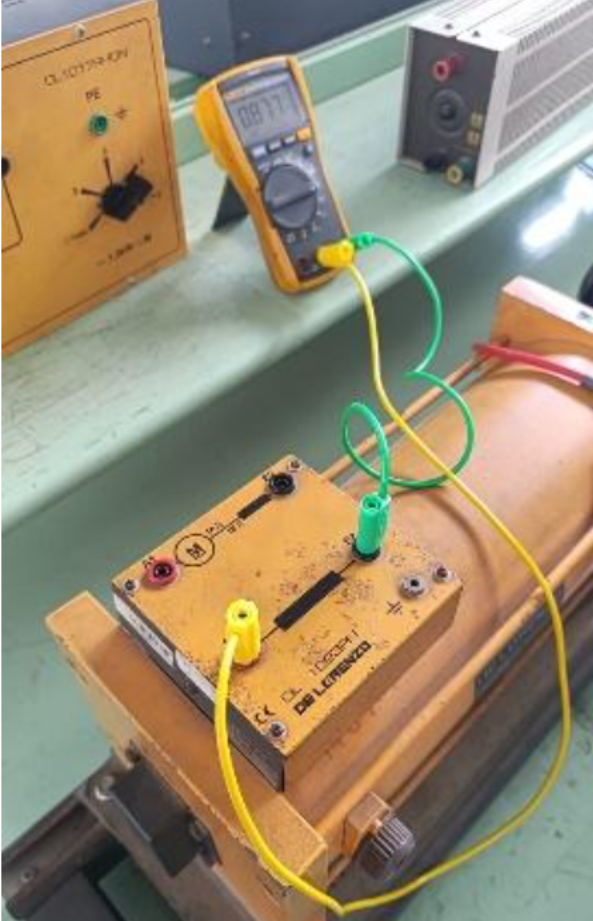
\includegraphics[width=0.48\textwidth, height=0.6\textwidth]{fot/Prac_6_A4.png}
    \caption{Montaje Resistencia de los devanados máquina shunt.}
    \label{fig:hoja}
\end{figure}

\begin{figure}[ht!]
    \centering
    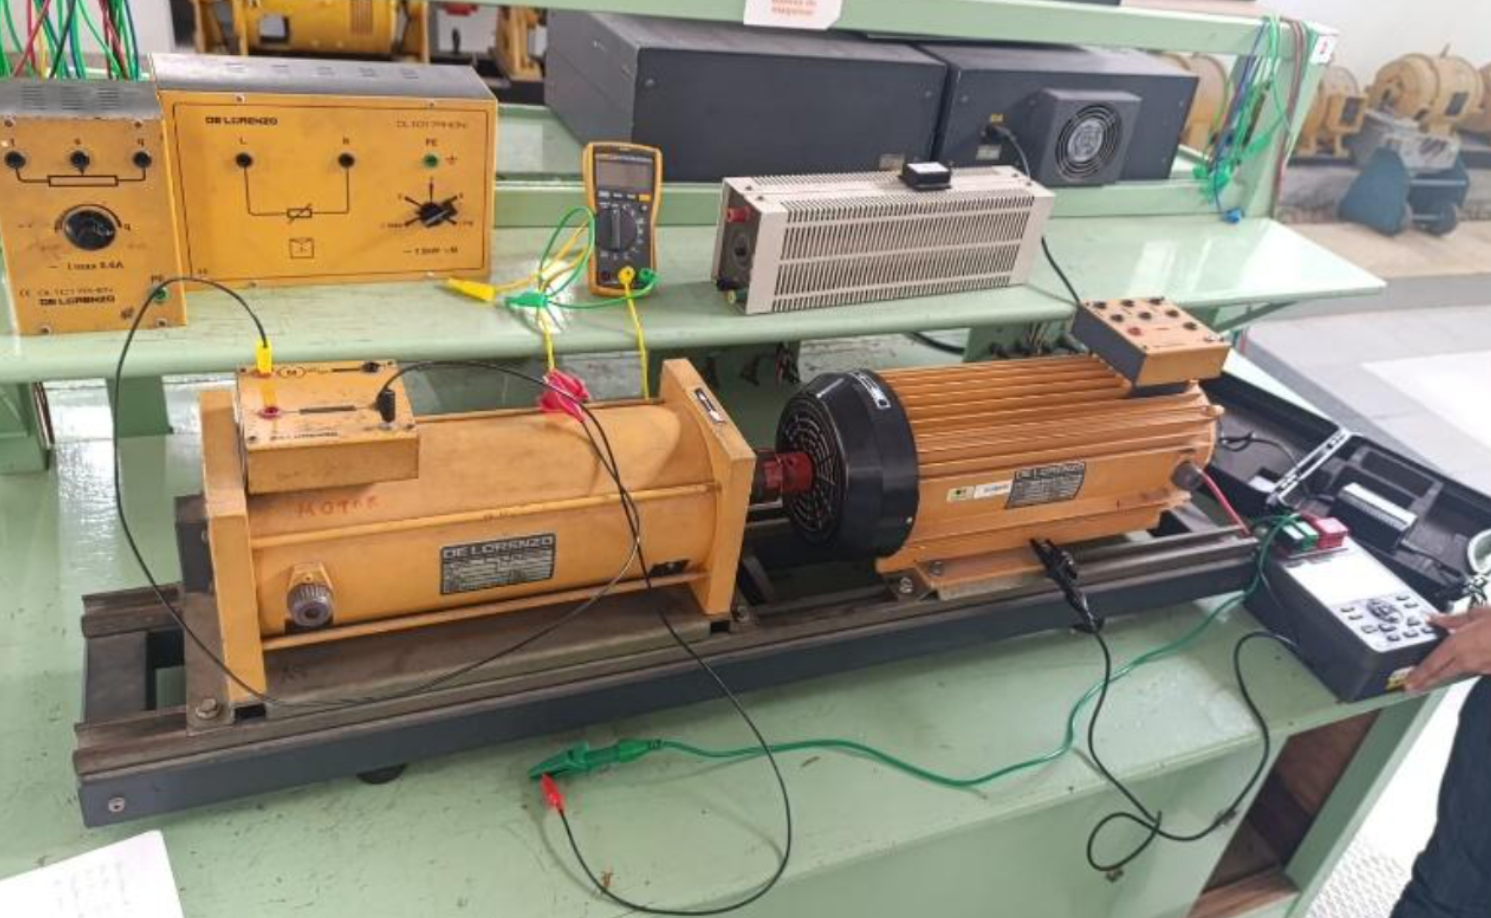
\includegraphics[width=0.48\textwidth]{fot/Prac_6_A2.png}
    \caption{Montaje resistencia de aislamiento.}
    \label{fig:A2}
\end{figure}


\begin{figure}[ht!]
    \centering
    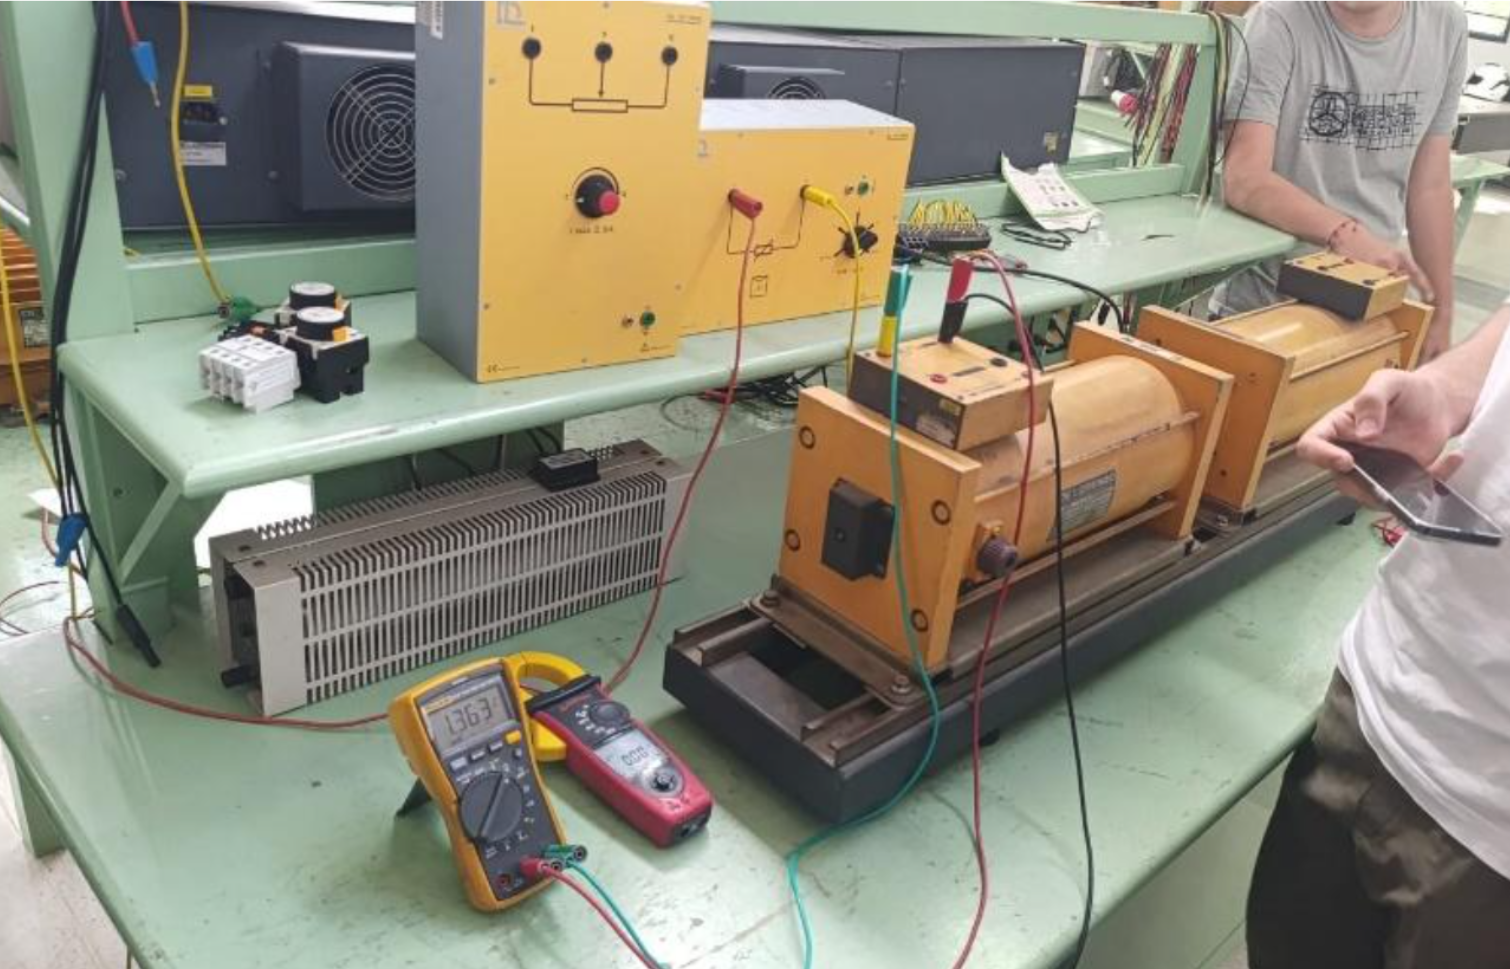
\includegraphics[width=0.48\textwidth]{fot/Prac_6_A1.png}
    \caption{Montaje prueba de caída de tensión en las escobillas.}
    \label{fig:A1}
\end{figure}



\subsection*{Hoja de datos}
\begin{figure}[ht!]
    \centering
    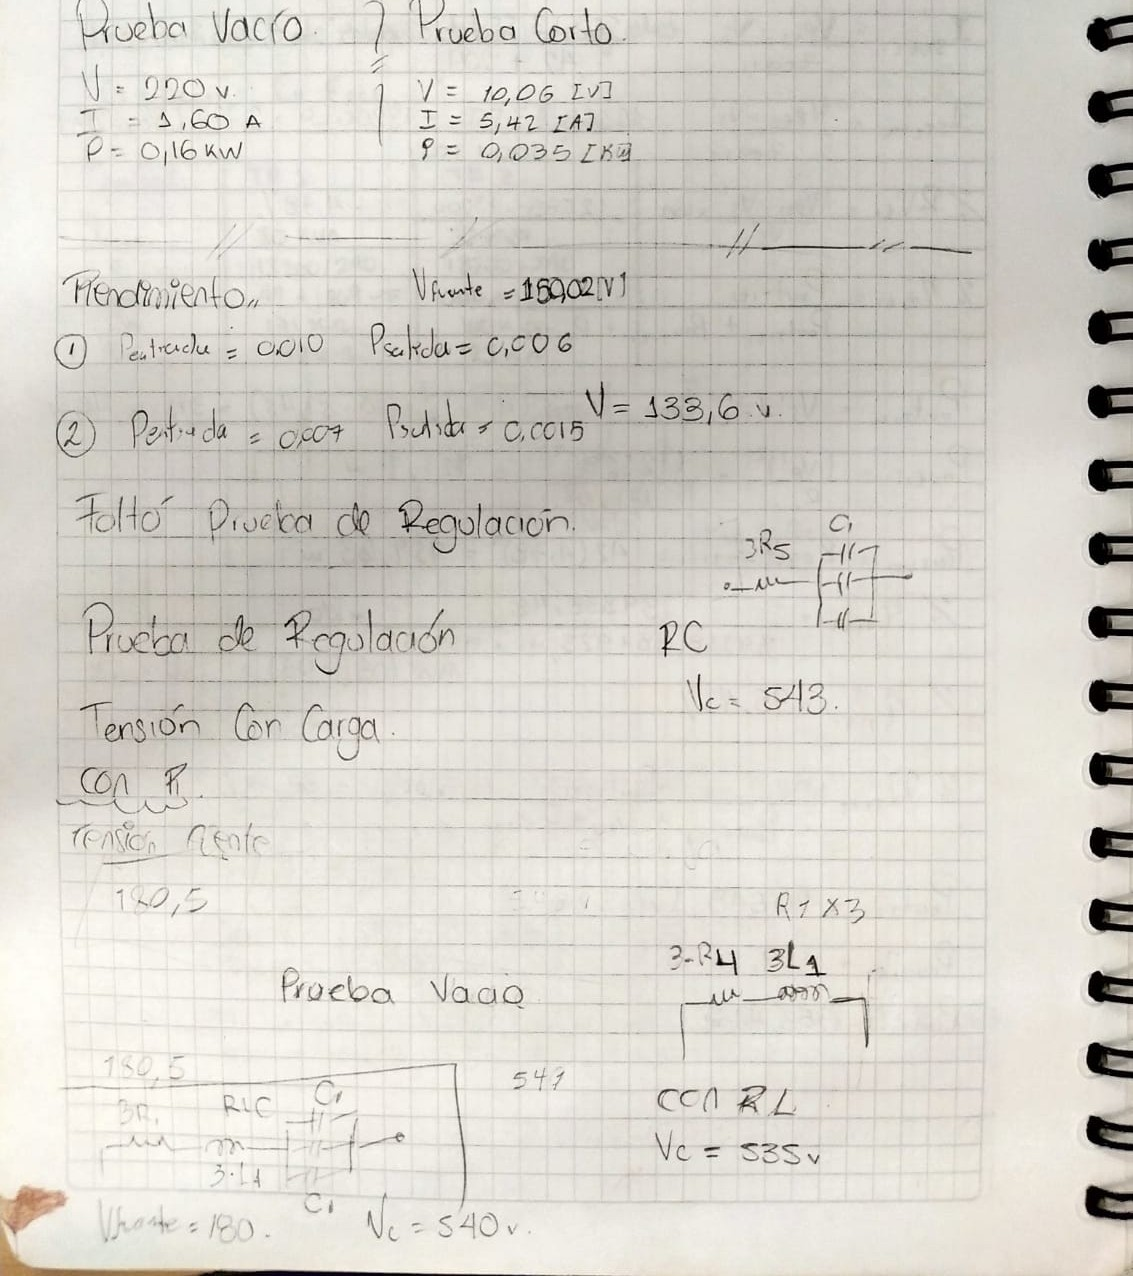
\includegraphics[width=0.48\textwidth]{fot/prac4_hoja de tales.jpg}
    \caption{Hoja de los datos tomados en el laboratorio.}
    \label{fig:A4}
\end{figure} %Anexos
         % Add the bibliography file in the preamble (correct usage)
        %\section*{Nomenclature}
        %    \addcontentsline{toc}{section}{Nomenclature}
        %    \begin{IEEEdescription}[\IEEEsetlabelwidth{$V_1,V_2,$}]
        %    \item[\smash{\begin{IEEEeqnarraybox*}[][t]{l}
        %    V_1,V_2,\\
        %    \hphantom{V_1,{}}V_3
        %    \end{IEEEeqnarraybox*}}] Three-phase PWM output line voltages.\\
        %    \mbox{}
        %    \item[$\theta$] Rotor angle (in ``electrical degrees'').
        %    \item[$\omega$] Rotor (electrical) speed, corresponding to the time
        %    derivative of $\theta$.
        %    \end{IEEEdescription}

        %    \begin{IEEEitemize}
        %        \item First item
        %        \item Second item
        %    \end{IEEEitemize}

            
        %    \begin{IEEEenumerate}
        %        \item First item
        %        \item Second item
        %    \end{IEEEenumerate}
        %    
        %    \begin{IEEEdescription}
        %        \item First item
        %        \item Second item
        %    \end{IEEEdescription}


        %   \begin{IEEEproof}
        %        The statement is true.
        %   \end{IEEEproof}


        \begin{thebibliography}{1}
            
            \bibitem{F1883}
            ASTM International, \emph{F1883 Standard Practice for Selection of Wire and Cable Size in AWG or Metric Units}, 1998. doi: 10.1520/F1883-98.
            \label{F1883}

            \bibitem{GonzalezGarcía2008}
            C. E. Gonzalez Aguas and O. García Colmenares, \emph{Guía para el diseño de núcleos de transformadores de distribución}, Trabajo de grado para optar al título de Ingeniero Electricista, Director H. R. Vargas Torres, Escuela de Ingenierías Eléctrica, Electrónica y Telecomunicaciones, Universidad Industrial de Santander, Bucaramanga, 2008.
            \label{GonzalezGarcía2008}

            \bibitem{Fraile2008}
            J. Fraile Mora, \emph{Máquinas Eléctricas}, 6ª ed. Madrid, España: McGraw-Hill, 2008.
            \label{Fraile2008}

        \end{thebibliography}

        \end{document}  
